% !TEX root = RRG_Report.tex
\documentclass[11pt,a4paper]{article}
\usepackage[margin=22mm,headheight=14pt]{geometry}
\usepackage{fontspec}
\setmainfont{Times New Roman}
\setsansfont{Arial}
\usepackage{amsmath,amssymb,float,graphicx,booktabs,longtable,array,caption,fancyhdr,xcolor,enumitem}
\usepackage[unicode,colorlinks=true,linkcolor=black,urlcolor=black,citecolor=black]{hyperref}
\definecolor{navy}{HTML}{171717}
\usepackage{titlesec}
\titleformat{\section}{\large\bfseries\color{navy}}{\thesection}{0.6em}{}
\titleformat{\subsection}{\normalsize\bfseries}{\thesubsection}{0.6em}{}
\titlespacing*{\section}{0pt}{10pt}{5pt}
\titlespacing*{\subsection}{0pt}{8pt}{4pt}
\setlength{\parindent}{0pt}
\setlength{\parskip}{5pt}
\linespread{1.04}
\setlength{\emergencystretch}{1.5em}
\captionsetup{font=small,labelfont=bf,skip=5pt}
\setlength{\tabcolsep}{5pt}
\renewcommand{\arraystretch}{1.13}
\pagestyle{fancy}\fancyhf{}
\fancyhead[L]{\small\sffamily RRG Sector Rotation | Empirical Analysis}
\fancyfoot[C]{\small\thepage}
\renewcommand{\headrulewidth}{0.3pt}
\setlist[itemize]{leftmargin=*,nosep,topsep=3pt}
\newcommand{\pp}{\,\text{pp}}

\hypersetup{pdftitle={Relative Strength and Sector Rotation in ETF Portfolios},pdfauthor={}}
\begin{document}
{\LARGE\bfseries Relative Strength and Sector Rotation in ETF Portfolios}\par
{\large Net Performance, Drawdown Risk, and Empirical Robustness}\par
{\small Portfolio Management Final Group Project \hfill 7 November 2026}

\section{Research question and strategy design}
This study evaluates the investment value of sector rotation based on the Relative Rotation Graph (RRG). The central question is whether a first-quadrant relative-strength rule improves net performance relative to a diffusion-plus-RRG strategy, conventional sector momentum, and an equal-weight ETF portfolio. We assess this question through a common portfolio construction and execution framework, with particular attention to the trade-off between compounded returns and drawdown risk.

Western Securities' May 2026 report [1] evaluates RRG quadrant portfolios at the sector-index level and implements a diffusion-plus-RRG ETF strategy. We extend its first-quadrant sector rule to the same ETF allocation framework. This extension permits a comparison of price-based relative strength with a composite signal that incorporates stock-level breadth. Disclosed fund holdings supply the sector exposures used in ETF implementation.

\subsection{Relative-strength signals}
RRG represents the level and evolution of relative strength. Let $P_{i,t}$ be sector $i$'s index level and $B_t$ an equally weighted, daily-compounded benchmark of 28 CITIC level-one sectors, excluding the two comprehensive categories. The implementation uses the following ratio construction:
\begin{align*}
RS_{i,t}&=100P_{i,t}/B_t,\\[-3pt]
R_{i,t}&=\operatorname{MA}_{20}\!\left(100RS_{i,t}/RS_{i,t-220}\right),\\[-3pt]
M_{i,t}&=\operatorname{MA}_{20}\!\left(100R_{i,t}/R_{i,t-60}\right).
\end{align*}
The horizontal coordinate $R$ measures the smoothed change in relative strength over 220 trading days; the vertical coordinate $M$ measures the subsequent change in that ratio over 60 days. The first quadrant requires $R>100$ and $M>100$. Computation follows the fixed implementation in [2]. Relative strength can improve while absolute returns remain negative, so the rule retains exposure to equity-market losses.

\subsection{Strategies and comparison portfolios}
\textbf{Pure RRG (Q)} selects up to six first-quadrant sectors, ranked by their Euclidean distance from $(100,100)$. \textbf{Diffusion + RRG (C)} first selects the six sectors with the highest smoothed, free-float-value-weighted share of stocks whose prices rose over 220 trading days; it then retains sectors in the first or second quadrant. The second quadrant has $R<100$ and $M>100$. Its final sector count can consequently fall below six.

\textbf{Sector momentum (M)} selects the six sectors with the highest 220-day index returns. It provides a parsimonious active benchmark under the same ETF implementation. \textbf{Equal-weight ETFs (E)} allocates equally across the same available ETF candidate pool each month, providing a diversified allocation benchmark. The RRG signal benchmark and the investable equal-weight ETF comparator serve separate purposes.

\newpage
\section{Data and portfolio implementation}
The evaluation runs from \textbf{28 December 2018 to 31 March 2026}, covering 1,756 trading days and 87 complete return months. Indicator warm-up begins on 3 January 2017; the first main-strategy trade occurs on 2 January 2019. Data include equity and sector-index prices, ETF prices and adjustment factors, historical sector membership, disclosed fund holdings, and product metadata. The data were obtained through an authorized Tushare-compatible interface [3]. Differences from the source report's Wind and Gildata inputs form part of the reconstruction uncertainty.

\subsection{ETF universe and portfolio construction}
The revised universe of industry and theme ETFs contains 718 products meeting type and date eligibility across the sample, including 54 products currently delisted. Historical eligibility, observed prices, visible holdings, overseas-holdings filtering, and turnover-based selection among ETFs tracking the same index determine the effective monthly pool. Its size rises from 48 products at the first formation date to 240 at the last.

Sector selection is followed by holdings-based ETF mapping, constrained optimization, and next-open rebalancing. The active strategies share the same exposure matrix and optimizer. Given the selected sectors, the optimizer maximizes total exposure to them, subject to full target investment, long-only ETF weights between zero and one, and an exposure cap of $1/k$ for each selected sector, where $k$ is the actual number selected. Thus, selecting six sectors can produce a different number of ETF positions and unequal ETF weights. Other sector exposures can enter through the ETFs' underlying holdings. The objective favors selected-sector exposure; transaction costs are charged during order execution.

\begin{table}[h]
\centering\small
\caption{Common backtest assumptions}
\begin{tabular}{@{}p{0.25\linewidth}p{0.69\linewidth}@{}}\toprule
Item & Setting \\\midrule
Signal and trading & Month-end close formation; next trading-day adjusted open execution; sales precede purchases; exited targets are set to zero.\\
Capital and costs & CNY 10 million initial capital; 3 basis points per side; zero additional slippage; zero cash yield.\\
Information and valuation & Holdings announced by formation; historical sector membership; adjusted close valuation; continuous fund units.\\
Performance conventions & 252 trading days per year; daily-return volatility and Sharpe ratio; zero risk-free rate for Sharpe.\\\bottomrule
\end{tabular}
\end{table}

\subsection{Data coverage and comparability}
Historical sector classification is incomplete early in the sample. Classified stocks cover approximately 56\% and 60\% of stock-days in 2018 and 2019, and 36\% and 42\% of free-float market value. The latter coverage reaches 98.66\% in 2020. Some ETF reports contain only their ten largest positions; disclosed and classified exposures retain their original net-asset-value weights. These limitations can affect breadth measures and ETF mapping differently across strategies.

The composite strategy is a reconstruction conditional on the available data. Its annualized return is 18.95\%, compared with 21.51\% in the original report. This gap combines data, universe, and implementation effects. The first-quadrant ETF strategy constitutes the application extension examined here. Appendix A documents data coverage, delisting conventions, and execution checks.

\newpage
\section{Performance and economic interpretation}
\begin{table}[h]
\centering\small
\caption{Portfolio performance after transaction costs}
\begin{tabular}{@{}lrrrr@{}}\toprule
Strategy & Ann. return & Ann. volatility & Sharpe & Max. drawdown\\\midrule
Pure RRG (Q) & 24.62\% & 26.36\% & 0.967 & $-44.76\%$\\
Diffusion + RRG (C) & 18.95\% & 27.02\% & 0.778 & $-38.40\%$\\
Sector momentum (M) & 21.83\% & 25.92\% & 0.892 & $-46.19\%$\\
Equal-weight ETFs (E) & 10.12\% & 19.68\% & 0.588 & $-38.78\%$\\\bottomrule
\end{tabular}
\end{table}

Pure RRG delivers the highest annualized return and Sharpe ratio under the main specification. Relative to momentum, its return increases by 2.79 percentage points, volatility increases slightly, and maximum drawdown improves by 1.44 percentage points. Terminal wealth from CNY 10 million is CNY 46.36 million, compared with CNY 39.58 million for momentum; these values include marked-to-market holdings.

\begin{figure}[h]
\centering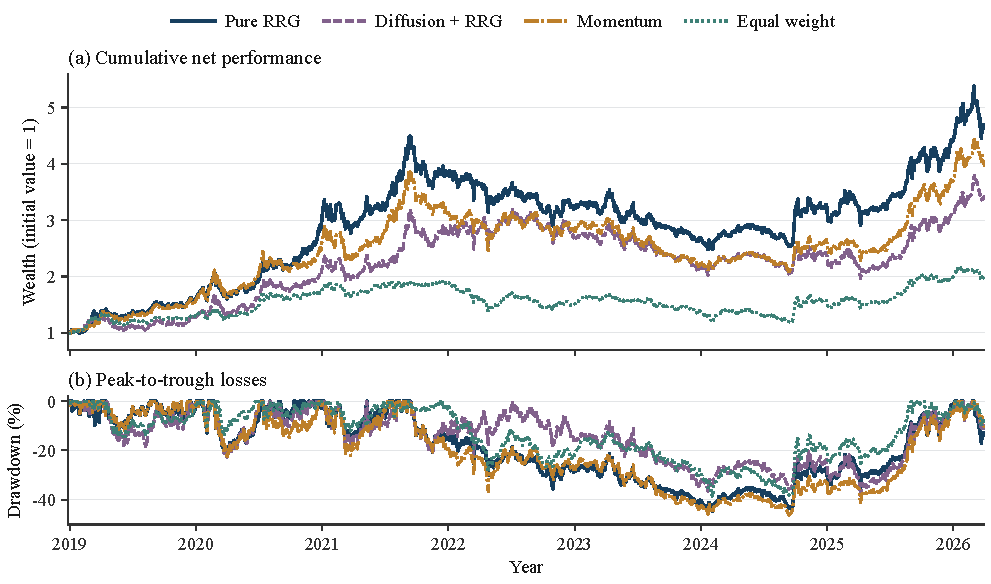
\includegraphics[width=\linewidth,height=0.39\textheight,keepaspectratio]{figures/01_net_nav.pdf}
\caption{Cumulative net performance and drawdown. Panel (a) reports wealth normalized to one at inception; Panel (b) reports losses relative to the running wealth maximum. The sample spans 28 December 2018--31 March 2026. All strategies use the common ETF pool and 3 bp one-way transaction costs.}
\end{figure}

Against the composite strategy, pure RRG gains 5.67 percentage points in annualized return while maximum drawdown deepens by 6.35 percentage points. The composite portfolio has the shallowest drawdown despite relatively high daily volatility. These rankings emphasize that return dispersion and cumulative losses along a particular path capture distinct dimensions of portfolio risk.

Equal weighting has the lowest volatility. Relative to this comparator, pure RRG combines stronger compounded growth with greater volatility and a deeper drawdown. Its Calmar ratio is 0.550, versus 0.473 for momentum and 0.493 for the composite strategy. The Q--C comparison jointly changes ranking, quadrant eligibility, and realized sector counts; it therefore evaluates complete allocation schemes. Identifying the marginal contribution of diffusion requires additional controls that hold those elements fixed.

\newpage
\section{Robustness and statistical inference}
\textbf{Time variation.} Across 76 overlapping 12-month windows, pure RRG exceeds momentum in 47, the composite strategy in 53, and equal weighting in 55; it ranks first in 29. Its calendar-year returns are $-16.47\%$ in 2022 and $-16.55\%$ in 2023. Window counts summarize the historical distribution of relative performance; adjacent observations share eleven months. The three strongest months account for 34.92\% of its total log growth. Mechanically setting each strategy's own best three months to zero leaves annualized returns of 15.40\% for Q and 13.67\% for M. This is a retrospective concentration diagnostic.

\textbf{Trading costs.} Replaying the target portfolios with one-way costs of 3, 5, 10, and 20 bp preserves Q's return advantage over M. At 20 bp, annualized returns are 21.49\% and 19.27\%, respectively. The main portfolio's annualized two-way turnover is approximately 14.97 times NAV, making execution relevant. These scenarios assess uniform friction; capacity depends on liquidity and capital-specific market impact.

\begin{figure}[h]
\centering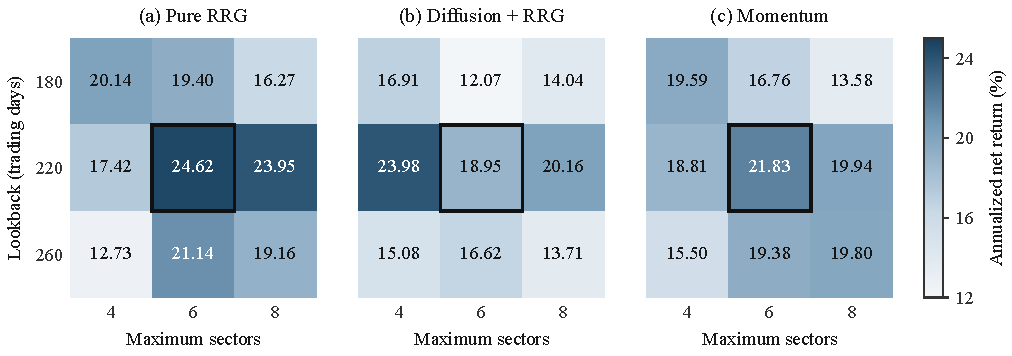
\includegraphics[width=0.98\linewidth,height=0.27\textheight,keepaspectratio]{figures/03_parameters.pdf}
\caption{Parameter sensitivity of annualized net returns (\%). Panels report Q, C, and M on a common color scale. Rows vary the signal lookback; columns vary the sector cap. The outlined cell identifies the main 220-day/six-sector specification. The 60-day momentum window, 20-day smoothing window, and 3 bp costs remain fixed.}
\end{figure}

\textbf{Parameters.} Across lookbacks of 180, 220, and 260 days and sector caps of four, six, and eight, Q exceeds matched-parameter M in six of nine cases, C in seven, and fixed E in all nine. Q's annualized return ranges from 12.73\% to 24.62\%. The main setting follows the adopted research configuration and also yields Q's highest return in the grid. Only two Q settings exceed the fixed main-setting momentum return. Parameter stability therefore depends on the comparison being made.

\textbf{Statistical inference.} Using 87 complete months, a paired mean net-return difference test with heteroskedasticity and autocorrelation consistent (HAC) standard errors at lag three gives $p=0.468$ for Q versus M. For Q versus E, the raw $p=0.017$ becomes $0.101$ after Holm adjustment across six primary comparisons. A three-month paired block bootstrap gives a 95\% interval of $[-4.85,10.76]$ percentage points for the Q--M annualized return gap. The observed economic return differences are therefore accompanied by substantial uncertainty about persistent incremental performance. Appendix D reports the complete tests and sensitivity checks.

\newpage
\section{Investor implications and limitations}
Pure first-quadrant RRG offers a favorable historical return--risk trade-off relative to momentum under the main specification. Its Sharpe ratio of 0.967 coexists with a maximum drawdown of 44.76\%, illustrating the distinction between average compensation for volatility and the loss an investor must withstand along the realized path. Relative to the composite scheme, the higher return entails a deeper drawdown. The evidence consequently supports evaluating RRG as a candidate active equity allocation for investors with a long horizon and substantial drawdown tolerance. Its role and weight within a broader portfolio depend on investor objectives and cross-asset covariances, which require a separate allocation analysis.

The trend-filter experiment further illustrates the importance of realized return paths. A common, fixed ten-month moving-average filter reduces Q's annualized return to 16.34\% and deepens its maximum drawdown to 47.04\%. Momentum experiences a similar deterioration. Lower volatility under the filter accompanies missed rebounds and delayed re-entry. Appendix E reports the complete comparison; the main analysis retains the unfiltered specification.

Several data and implementation features qualify the results. Early sector-membership gaps affect the inputs to diffusion and ETF exposures. Partial holdings disclosure means the optimizer acts on observed exposures, while current index-category labels and incomplete historical product identities can influence the reconstructed universe. Delisted funds are included, with cash settlement approximated using previously announced NAV at the first monthly formation on or after delisting. The main equal-weight portfolio has 25 estimated settlements, while the three main active portfolios have zero. This asymmetry matters when interpreting their comparison.

Trading uses continuous units and adjusted opening prices, with costs applied proportionally. Practical implementation additionally requires lot sizes, minimum commissions, opening-market liquidity, and actual liquidation cash flows. The analysis uses one already-observed historical sample, and the multiple-testing adjustments cover the specified comparison families. Independent future observations and more complete point-in-time data would strengthen inference about persistent value.

\textbf{Conclusion.} The first-quadrant rule produces favorable historical net performance within the common ETF framework. This economic advantage is accompanied by substantial drawdown risk and imprecisely estimated incremental returns. The findings identify an empirically promising sector-allocation rule and establish the conditions under which its historical performance is relevant. More complete point-in-time inputs and independent observations are central to assessing its persistent investment value.

\section*{References}
\begingroup\footnotesize\setlength{\parskip}{3pt}
[1] Western Securities Research Center (2026). \emph{Index-based Allocation Research Series (6): Sector Research under the Relative Rotation Graph Framework}. 25 May. Chinese report; Sections 2.1 and 3.1; Table 13.

[2] hugo2046. \emph{QuantsPlaybook}, RRG sector-rotation implementation. Fixed commit \texttt{3f83a77f4c79} (full hash in the appendix). \url{https://github.com/hugo2046/QuantsPlaybook}.

[3] Tushare-compatible data interface. Equity, CITIC sector, index, ETF, fund-holdings and NAV datasets; locally archived inputs. Data-provider equivalence and historical coverage are discussed in Section 2 and Appendix A.

\textit{Companion technical appendix:} complete cost, parameter, inference and moving-average results; data conventions; reproducibility index. Figures are rendered as vector graphics from the archived results.
\endgroup
\end{document}
